\pdfoutput=1
%% Author: PGL  Porta Mana
%% Created: 2019-03-23T19:34:27+0100
%% Last-Updated: 2023-05-04T13:16:39+0200
%%%%%%%%%%%%%%%%%%%%%%%%%%%%%%%%%%%%%%%%%%%%%%%%%%%%%%%%%%%%%%%%%%%%%%%%%%%%
\newif\ifarxiv
\arxivfalse
\ifarxiv\pdfmapfile{+classico.map}\fi
\newif\ifafour
\afourfalse% true = A4, false = A5
\newif\iftypodisclaim % typographical disclaim on the side
\typodisclaimtrue
\newcommand*{\memfontfamily}{zplx}
\newcommand*{\memfontpack}{newpxtext}
\documentclass[\ifafour a4paper,12pt,\else a5paper,10pt,\fi%extrafontsizes,%
onecolumn,oneside,article,%french,italian,german,swedish,latin,
british%
]{memoir}
\newcommand*{\updated}{\today}
\newcommand*{\firstdraft}{23 March 2019}
\newcommand*{\firstpublished}{23 March 2019}
\newcommand*{\propertitle}{Introduction to probability 2\\ Exercise: the Monty Hall problem%\\{\large ***}%
}
\newcommand*{\pdftitle}{Introduction to probability 2 -- Exercise: the Monty Hall problem}
\newcommand*{\headtitle}{Exercise 2: Monty Hall}
\newcommand*{\pdfauthor}{P.G.L.  Porta Mana}
\newcommand*{\headauthor}{Intro to probability 2}
\newcommand*{\reporthead}{}% Report number

%%%%%%%%%%%%%%%%%%%%%%%%%%%%%%%%%%%%%%%%%%%%%%%%%%%%%%%%%%%%%%%%%%%%%%%%%%%%
%%% Calls to packages (uncomment as needed)
%%%%%%%%%%%%%%%%%%%%%%%%%%%%%%%%%%%%%%%%%%%%%%%%%%%%%%%%%%%%%%%%%%%%%%%%%%%%

%\usepackage{pifont}

%\usepackage{fontawesome}

\usepackage[T1]{fontenc} 
\input{glyphtounicode} \pdfgentounicode=1

\usepackage[utf8]{inputenx}

%\usepackage{newunicodechar}
% \newunicodechar{Ĕ}{\u{E}}
% \newunicodechar{ĕ}{\u{e}}
% \newunicodechar{Ĭ}{\u{I}}
% \newunicodechar{ĭ}{\u{\i}}
% \newunicodechar{Ŏ}{\u{O}}
% \newunicodechar{ŏ}{\u{o}}
% \newunicodechar{Ŭ}{\u{U}}
% \newunicodechar{ŭ}{\u{u}}
% \newunicodechar{Ā}{\=A}
% \newunicodechar{ā}{\=a}
% \newunicodechar{Ē}{\=E}
% \newunicodechar{ē}{\=e}
% \newunicodechar{Ī}{\=I}
% \newunicodechar{ī}{\={\i}}
% \newunicodechar{Ō}{\=O}
% \newunicodechar{ō}{\=o}
% \newunicodechar{Ū}{\=U}
% \newunicodechar{ū}{\=u}
% \newunicodechar{Ȳ}{\=Y}
% \newunicodechar{ȳ}{\=y}

\newcommand*{\bmmax}{0} % reduce number of bold fonts, before font packages
\newcommand*{\hmmax}{0} % reduce number of heavy fonts, before font packages

\usepackage{textcomp}

%\usepackage[normalem]{ulem}% package for underlining
% \makeatletter
% \def\ssout{\bgroup \ULdepth=-.35ex%\UL@setULdepth
%  \markoverwith{\lower\ULdepth\hbox
%    {\kern-.03em\vbox{\hrule width.2em\kern1.2\p@\hrule}\kern-.03em}}%
%  \ULon}
% \makeatother

\usepackage{amsmath}

\usepackage{mathtools}
\addtolength{\jot}{\jot} % increase spacing in multiline formulae
\setlength{\multlinegap}{0pt}

%\usepackage{empheq}% automatically calls amsmath and mathtools
\newcommand*{\widefbox}[1]{\fbox{\hspace{1em}#1\hspace{1em}}}

%\usepackage{fancybox}

\usepackage{framed}

% \usepackage[misc]{ifsym} % for dice
% \newcommand*{\diceone}{{\scriptsize\Cube{1}}}

\usepackage{amssymb}

\usepackage{amsxtra}

\usepackage[main=british,french,italian,german,swedish,latin,esperanto]{babel}\selectlanguage{british}
\newcommand*{\langfrench}{\foreignlanguage{french}}
\newcommand*{\langgerman}{\foreignlanguage{german}}
\newcommand*{\langitalian}{\foreignlanguage{italian}}
\newcommand*{\langswedish}{\foreignlanguage{swedish}}
\newcommand*{\langlatin}{\foreignlanguage{latin}}
\newcommand*{\langnohyph}{\foreignlanguage{nohyphenation}}

\usepackage[autostyle=false,autopunct=false,english=british]{csquotes}
\setquotestyle{british}
\newcommand*{\defquote}[1]{``#1''}

\usepackage{amsthm}
\newcommand*{\QED}{\textsc{q.e.d.}}
\renewcommand*{\qedsymbol}{\QED}
\theoremstyle{remark}
\newtheorem{note}{Note}
\newtheorem*{remark}{Note}
\newtheoremstyle{innote}{\parsep}{\parsep}{\footnotesize}{}{}{}{0pt}{}
\theoremstyle{innote}
\newtheorem*{innote}{}

\usepackage[shortlabels,inline]{enumitem}
\SetEnumitemKey{para}{itemindent=\parindent,leftmargin=0pt,listparindent=\parindent,parsep=0pt,itemsep=\topsep}
% \begin{asparaenum} = \begin{enumerate}[para]
% \begin{inparaenum} = \begin{enumerate*}
\setlist[enumerate,2]{label=\alph*.}
\setlist[enumerate]{label=\arabic*.,leftmargin=1.5\parindent}
\setlist[itemize]{leftmargin=1.5\parindent}
\setlist[description]{leftmargin=1.5\parindent}
% old alternative:
% \setlist[enumerate,2]{label=\alph*.}
% \setlist[enumerate]{leftmargin=\parindent}
% \setlist[itemize]{leftmargin=\parindent}
% \setlist[description]{leftmargin=\parindent}

\usepackage[babel,theoremfont,largesc]{newpxtext}

\usepackage[bigdelims,nosymbolsc%,smallerops % probably arXiv doesn't have it
]{newpxmath}
\useosf\linespread{1.083}
%% smaller operators for old version of newpxmath
\makeatletter
\def\re@DeclareMathSymbol#1#2#3#4{%
    \let#1=\undefined
    \DeclareMathSymbol{#1}{#2}{#3}{#4}}
%\re@DeclareMathSymbol{\bigsqcupop}{\mathop}{largesymbols}{"46}
%\re@DeclareMathSymbol{\bigodotop}{\mathop}{largesymbols}{"4A}
\re@DeclareMathSymbol{\bigoplusop}{\mathop}{largesymbols}{"4C}
\re@DeclareMathSymbol{\bigotimesop}{\mathop}{largesymbols}{"4E}
\re@DeclareMathSymbol{\sumop}{\mathop}{largesymbols}{"50}
\re@DeclareMathSymbol{\prodop}{\mathop}{largesymbols}{"51}
\re@DeclareMathSymbol{\bigcupop}{\mathop}{largesymbols}{"53}
\re@DeclareMathSymbol{\bigcapop}{\mathop}{largesymbols}{"54}
%\re@DeclareMathSymbol{\biguplusop}{\mathop}{largesymbols}{"55}
\re@DeclareMathSymbol{\bigwedgeop}{\mathop}{largesymbols}{"56}
\re@DeclareMathSymbol{\bigveeop}{\mathop}{largesymbols}{"57}
%\re@DeclareMathSymbol{\bigcupdotop}{\mathop}{largesymbols}{"DF}
%\re@DeclareMathSymbol{\bigcapplusop}{\mathop}{largesymbolsPXA}{"00}
%\re@DeclareMathSymbol{\bigsqcupplusop}{\mathop}{largesymbolsPXA}{"02}
%\re@DeclareMathSymbol{\bigsqcapplusop}{\mathop}{largesymbolsPXA}{"04}
%\re@DeclareMathSymbol{\bigsqcapop}{\mathop}{largesymbolsPXA}{"06}
\re@DeclareMathSymbol{\bigtimesop}{\mathop}{largesymbolsPXA}{"10}
%\re@DeclareMathSymbol{\coprodop}{\mathop}{largesymbols}{"60}
%\re@DeclareMathSymbol{\varprod}{\mathop}{largesymbolsPXA}{16}
\makeatother
%%
%% With euler font cursive for Greek letters - the [1] means 100% scaling
\DeclareFontFamily{U}{egreek}{\skewchar\font'177}%
\DeclareFontShape{U}{egreek}{m}{n}{<-6>s*[1]eurm5 <6-8>s*[1]eurm7 <8->s*[1]eurm10}{}%
\DeclareFontShape{U}{egreek}{m}{it}{<->s*[1]eurmo10}{}%
\DeclareFontShape{U}{egreek}{b}{n}{<-6>s*[1]eurb5 <6-8>s*[1]eurb7 <8->s*[1]eurb10}{}%
\DeclareFontShape{U}{egreek}{b}{it}{<->s*[1]eurbo10}{}%
\DeclareSymbolFont{egreeki}{U}{egreek}{m}{it}%
\SetSymbolFont{egreeki}{bold}{U}{egreek}{b}{it}% from the amsfonts package
\DeclareSymbolFont{egreekr}{U}{egreek}{m}{n}%
\SetSymbolFont{egreekr}{bold}{U}{egreek}{b}{n}% from the amsfonts package
% Take also \sum, \prod, \coprod symbols from Euler fonts
\DeclareFontFamily{U}{egreekx}{\skewchar\font'177}
\DeclareFontShape{U}{egreekx}{m}{n}{%
       <-7.5>s*[0.9]euex7%
    <7.5-8.5>s*[0.9]euex8%
    <8.5-9.5>s*[0.9]euex9%
    <9.5->s*[0.9]euex10%
}{}
\DeclareSymbolFont{egreekx}{U}{egreekx}{m}{n}
\DeclareMathSymbol{\sumop}{\mathop}{egreekx}{"50}
\DeclareMathSymbol{\prodop}{\mathop}{egreekx}{"51}
\DeclareMathSymbol{\coprodop}{\mathop}{egreekx}{"60}
\makeatletter
\def\sum{\DOTSI\sumop\slimits@}
\def\prod{\DOTSI\prodop\slimits@}
\def\coprod{\DOTSI\coprodop\slimits@}
\makeatother
% Greek letters not usually given in LaTeX.
\DeclareMathSymbol{\varpartial}{\mathalpha}{egreeki}{"40}
\DeclareMathSymbol{\partialup}{\mathalpha}{egreekr}{"40}
\DeclareMathSymbol{\alpha}{\mathalpha}{egreeki}{"0B}
\DeclareMathSymbol{\beta}{\mathalpha}{egreeki}{"0C}
\DeclareMathSymbol{\gamma}{\mathalpha}{egreeki}{"0D}
\DeclareMathSymbol{\delta}{\mathalpha}{egreeki}{"0E}
\DeclareMathSymbol{\epsilon}{\mathalpha}{egreeki}{"0F}
\DeclareMathSymbol{\zeta}{\mathalpha}{egreeki}{"10}
\DeclareMathSymbol{\eta}{\mathalpha}{egreeki}{"11}
\DeclareMathSymbol{\theta}{\mathalpha}{egreeki}{"12}
\DeclareMathSymbol{\iota}{\mathalpha}{egreeki}{"13}
\DeclareMathSymbol{\kappa}{\mathalpha}{egreeki}{"14}
\DeclareMathSymbol{\lambda}{\mathalpha}{egreeki}{"15}
\DeclareMathSymbol{\mu}{\mathalpha}{egreeki}{"16}
\DeclareMathSymbol{\nu}{\mathalpha}{egreeki}{"17}
\DeclareMathSymbol{\xi}{\mathalpha}{egreeki}{"18}
\DeclareMathSymbol{\omicron}{\mathalpha}{egreeki}{"6F}
\DeclareMathSymbol{\pi}{\mathalpha}{egreeki}{"19}
\DeclareMathSymbol{\rho}{\mathalpha}{egreeki}{"1A}
\DeclareMathSymbol{\sigma}{\mathalpha}{egreeki}{"1B}
 \DeclareMathSymbol{\tau}{\mathalpha}{egreeki}{"1C}
\DeclareMathSymbol{\upsilon}{\mathalpha}{egreeki}{"1D}
\DeclareMathSymbol{\phi}{\mathalpha}{egreeki}{"1E}
\DeclareMathSymbol{\chi}{\mathalpha}{egreeki}{"1F}
\DeclareMathSymbol{\psi}{\mathalpha}{egreeki}{"20}
\DeclareMathSymbol{\omega}{\mathalpha}{egreeki}{"21}
\DeclareMathSymbol{\varepsilon}{\mathalpha}{egreeki}{"22}
\DeclareMathSymbol{\vartheta}{\mathalpha}{egreeki}{"23}
\DeclareMathSymbol{\varpi}{\mathalpha}{egreeki}{"24}
\let\varrho\rho 
\let\varsigma\sigma
 \let\varkappa\kappa
\DeclareMathSymbol{\varphi}{\mathalpha}{egreeki}{"27}
%
\DeclareMathSymbol{\varAlpha}{\mathalpha}{egreeki}{"41}
\DeclareMathSymbol{\varBeta}{\mathalpha}{egreeki}{"42}
\DeclareMathSymbol{\varGamma}{\mathalpha}{egreeki}{"00}
\DeclareMathSymbol{\varDelta}{\mathalpha}{egreeki}{"01}
\DeclareMathSymbol{\varEpsilon}{\mathalpha}{egreeki}{"45}
\DeclareMathSymbol{\varZeta}{\mathalpha}{egreeki}{"5A}
\DeclareMathSymbol{\varEta}{\mathalpha}{egreeki}{"48}
\DeclareMathSymbol{\varTheta}{\mathalpha}{egreeki}{"02}
 \DeclareMathSymbol{\varIota}{\mathalpha}{egreeki}{"49}
\DeclareMathSymbol{\varKappa}{\mathalpha}{egreeki}{"4B}
\DeclareMathSymbol{\varLambda}{\mathalpha}{egreeki}{"03}
\DeclareMathSymbol{\varMu}{\mathalpha}{egreeki}{"4D}
\DeclareMathSymbol{\varNu}{\mathalpha}{egreeki}{"4E}
\DeclareMathSymbol{\varXi}{\mathalpha}{egreeki}{"04}
\DeclareMathSymbol{\varOmicron}{\mathalpha}{egreeki}{"4F}
\DeclareMathSymbol{\varPi}{\mathalpha}{egreeki}{"05}
\DeclareMathSymbol{\varRho}{\mathalpha}{egreeki}{"50}
\DeclareMathSymbol{\varSigma}{\mathalpha}{egreeki}{"06}
\DeclareMathSymbol{\varTau}{\mathalpha}{egreeki}{"54}
\DeclareMathSymbol{\varUpsilon}{\mathalpha}{egreeki}{"07}
\DeclareMathSymbol{\varPhi}{\mathalpha}{egreeki}{"08}
\DeclareMathSymbol{\varChi}{\mathalpha}{egreeki}{"58}
\DeclareMathSymbol{\varPsi}{\mathalpha}{egreeki}{"09}
\DeclareMathSymbol{\varOmega}{\mathalpha}{egreeki}{"0A} 
%
\DeclareMathSymbol{\Alpha}{\mathalpha}{egreekr}{"41}
\DeclareMathSymbol{\Beta}{\mathalpha}{egreekr}{"42}
\DeclareMathSymbol{\Gamma}{\mathalpha}{egreekr}{"00}
\DeclareMathSymbol{\Delta}{\mathalpha}{egreekr}{"01}
\DeclareMathSymbol{\Epsilon}{\mathalpha}{egreekr}{"45}
\DeclareMathSymbol{\Zeta}{\mathalpha}{egreekr}{"5A}
\DeclareMathSymbol{\Eta}{\mathalpha}{egreekr}{"48}
\DeclareMathSymbol{\Theta}{\mathalpha}{egreekr}{"02}
\DeclareMathSymbol{\Iota}{\mathalpha}{egreekr}{"49}
\DeclareMathSymbol{\Kappa}{\mathalpha}{egreekr}{"4B}
\DeclareMathSymbol{\Lambda}{\mathalpha}{egreekr}{"03}
\DeclareMathSymbol{\Mu}{\mathalpha}{egreekr}{"4D}
\DeclareMathSymbol{\Nu}{\mathalpha}{egreekr}{"4E}
\DeclareMathSymbol{\Xi}{\mathalpha}{egreekr}{"04}
\DeclareMathSymbol{\Omicron}{\mathalpha}{egreekr}{"4F}
\DeclareMathSymbol{\Pi}{\mathalpha}{egreekr}{"05}
\DeclareMathSymbol{\Rho}{\mathalpha}{egreekr}{"50}
\DeclareMathSymbol{\Sigma}{\mathalpha}{egreekr}{"06}
\DeclareMathSymbol{\Tau}{\mathalpha}{egreekr}{"54}
\DeclareMathSymbol{\Upsilon}{\mathalpha}{egreekr}{"07}
\DeclareMathSymbol{\Phi}{\mathalpha}{egreekr}{"08}
\DeclareMathSymbol{\Chi}{\mathalpha}{egreekr}{"58}
\DeclareMathSymbol{\Psi}{\mathalpha}{egreekr}{"09}
\DeclareMathSymbol{\Omega}{\mathalpha}{egreekr}{"0A}
%
\DeclareMathSymbol{\alphaup}{\mathalpha}{egreekr}{"0B}
\DeclareMathSymbol{\betaup}{\mathalpha}{egreekr}{"0C}
\DeclareMathSymbol{\gammaup}{\mathalpha}{egreekr}{"0D}
 \DeclareMathSymbol{\deltaup}{\mathalpha}{egreekr}{"0E}
\DeclareMathSymbol{\epsilonup}{\mathalpha}{egreekr}{"0F}
\DeclareMathSymbol{\zetaup}{\mathalpha}{egreekr}{"10}
\DeclareMathSymbol{\etaup}{\mathalpha}{egreekr}{"11}
\DeclareMathSymbol{\thetaup}{\mathalpha}{egreekr}{"12}
\DeclareMathSymbol{\iotaup}{\mathalpha}{egreekr}{"13}
\DeclareMathSymbol{\kappaup}{\mathalpha}{egreekr}{"14}
\DeclareMathSymbol{\lambdaup}{\mathalpha}{egreekr}{"15}
\DeclareMathSymbol{\muup}{\mathalpha}{egreekr}{"16}
\DeclareMathSymbol{\nuup}{\mathalpha}{egreekr}{"17}
\DeclareMathSymbol{\xiup}{\mathalpha}{egreekr}{"18}
\DeclareMathSymbol{\omicronup}{\mathalpha}{egreekr}{"6F}
  \DeclareMathSymbol{\piup}{\mathalpha}{egreekr}{"19}
\DeclareMathSymbol{\rhoup}{\mathalpha}{egreekr}{"1A}
\DeclareMathSymbol{\sigmaup}{\mathalpha}{egreekr}{"1B}
\DeclareMathSymbol{\tauup}{\mathalpha}{egreekr}{"1C}
\DeclareMathSymbol{\upsilonup}{\mathalpha}{egreekr}{"1D}
\DeclareMathSymbol{\phiup}{\mathalpha}{egreekr}{"1E}
\DeclareMathSymbol{\chiup}{\mathalpha}{egreekr}{"1F}
\DeclareMathSymbol{\psiup}{\mathalpha}{egreekr}{"20}
\DeclareMathSymbol{\omegaup}{\mathalpha}{egreekr}{"21}
\DeclareMathSymbol{\varepsilonup}{\mathalpha}{egreekr}{"22}
\DeclareMathSymbol{\varthetaup}{\mathalpha}{egreekr}{"23}
\DeclareMathSymbol{\varpiup}{\mathalpha}{egreekr}{"24}
\let\varrhoup\rhoup 
\let\varsigmaup\sigmaup
\let\varkappaup\kappaup
\DeclareMathSymbol{\varphiup}{\mathalpha}{egreekr}{"27}
% Greek letters not usually given in LaTeX.

%\usepackage%[scaled=0.9]%
%{classico}%  Optima as sans-serif font
\renewcommand\sfdefault{uop}
\DeclareMathAlphabet{\mathsf}  {T1}{\sfdefault}{m}{sl}
\SetMathAlphabet{\mathsf}{bold}{T1}{\sfdefault}{b}{sl}
%\newcommand*{\mathte}[1]{\textbf{\textit{\textsf{#1}}}}
% Upright sans-serif math alphabet
% \DeclareMathAlphabet{\mathsu}  {T1}{\sfdefault}{m}{n}
% \SetMathAlphabet{\mathsu}{bold}{T1}{\sfdefault}{b}{n}

% DejaVu Mono as typewriter text
\usepackage[scaled=0.84]{DejaVuSansMono}

\usepackage{mathdots}

\usepackage[usenames]{xcolor}
% Tol (2012) colour-blind-, print-, screen-friendly colours, alternative scheme; Munsell terminology
\definecolor{mypurpleblue}{RGB}{68,119,170}
\definecolor{myblue}{RGB}{102,204,238}
\definecolor{mygreen}{RGB}{34,136,51}
\definecolor{myyellow}{RGB}{204,187,68}
\definecolor{myred}{RGB}{238,102,119}
\definecolor{myredpurple}{RGB}{170,51,119}
\definecolor{mygrey}{RGB}{187,187,187}
% Tol (2012) colour-blind-, print-, screen-friendly colours; Munsell terminology
% \definecolor{lbpurple}{RGB}{51,34,136}
% \definecolor{lblue}{RGB}{136,204,238}
% \definecolor{lbgreen}{RGB}{68,170,153}
% \definecolor{lgreen}{RGB}{17,119,51}
% \definecolor{lgyellow}{RGB}{153,153,51}
% \definecolor{lyellow}{RGB}{221,204,119}
% \definecolor{lred}{RGB}{204,102,119}
% \definecolor{lpred}{RGB}{136,34,85}
% \definecolor{lrpurple}{RGB}{170,68,153}
\definecolor{lgrey}{RGB}{221,221,221}
%\newcommand*\mycolourbox[1]{%
%\colorbox{mygrey}{\hspace{1em}#1\hspace{1em}}}
\colorlet{shadecolor}{lgrey}

\usepackage{bm}

\usepackage{microtype}

\usepackage[backend=biber,mcite,%subentry,
citestyle=authoryear-comp,bibstyle=pglpm-authoryear,autopunct=false,sorting=ny,sortcites=false,natbib=false,maxcitenames=1,maxbibnames=8,minbibnames=8,giveninits=true,uniquename=false,uniquelist=false,maxalphanames=1,block=space,hyperref=true,defernumbers=false,useprefix=true,sortupper=false,language=british,parentracker=false]{biblatex}
\DeclareSortingScheme{ny}{\sort{\field{sortname}\field{author}\field{editor}}\sort{\field{year}}}
\iffalse\makeatletter%%% replace parenthesis with brackets
\newrobustcmd*{\parentexttrack}[1]{%
  \begingroup
  \blx@blxinit
  \blx@setsfcodes
  \blx@bibopenparen#1\blx@bibcloseparen
  \endgroup}
\AtEveryCite{%
  \let\parentext=\parentexttrack%
  \let\bibopenparen=\bibopenbracket%
  \let\bibcloseparen=\bibclosebracket}
\makeatother\fi
\DefineBibliographyExtras{british}{\def\finalandcomma{\addcomma}}
\renewcommand*{\finalnamedelim}{\addcomma\space}
\setcounter{biburlnumpenalty}{1}
\setcounter{biburlucpenalty}{0}
\setcounter{biburllcpenalty}{1}
\DeclareDelimFormat{multicitedelim}{\addsemicolon\space}
\DeclareDelimFormat{compcitedelim}{\addsemicolon\space}
\DeclareDelimFormat{postnotedelim}{\space}
\ifarxiv\else\addbibresource{portamanabib.bib}\fi
\renewcommand{\bibfont}{\footnotesize}
%\appto{\citesetup}{\footnotesize}% smaller font for citations
\defbibheading{bibliography}[\bibname]{\section*{#1}\addcontentsline{toc}{section}{#1}%\markboth{#1}{#1}
}
\newcommand*{\citep}{\parencites}
\newcommand*{\citey}{\parencites*}
%\renewcommand*{\cite}{\parencite}
\renewcommand*{\cites}{\parencites}
\providecommand{\href}[2]{#2}
\providecommand{\eprint}[2]{\texttt{\href{#1}{#2}}}
\newcommand*{\ibid}{\unspace\addtocounter{footnote}{-1}\footnotemark{}}
\newcommand*{\amp}{\&}
% \newcommand*{\citein}[2][]{\textnormal{\textcite[#1]{#2}}%\addtocategory{extras}{#2}
% }
\newcommand*{\citein}[2][]{\textnormal{\textcite[#1]{#2}}%\addtocategory{extras}{#2}
}
\newcommand*{\citebi}[2][]{\textcite[#1]{#2}%\addtocategory{extras}{#2}
}
\newcommand*{\subtitleproc}[1]{}
\newcommand*{\chapb}{ch.}
%
% \def\arxivp{}
% \def\mparcp{}
% \def\philscip{}
% \def\biorxivp{}
% \newcommand*{\arxivsi}{\texttt{arXiv} eprints available at \url{http://arxiv.org/}.\\}
% \newcommand*{\mparcsi}{\texttt{mp\_arc} eprints available at \url{http://www.ma.utexas.edu/mp_arc/}.\\}
% \newcommand*{\philscisi}{\texttt{philsci} eprints available at \url{http://philsci-archive.pitt.edu/}.\\}
% \newcommand*{\biorxivsi}{\texttt{bioRxiv} eprints available at \url{http://biorxiv.org/}.\\}
\newcommand*{\arxiveprint}[1]{%\global\def\arxivp{\arxivsi}%\citeauthor{0arxivcite}\addtocategory{ifarchcit}{0arxivcite}%eprint
\texttt{\urlalt{https://arxiv.org/abs/#1}{arXiv:\hspace{0pt}#1}}%
%\texttt{\href{http://arxiv.org/abs/#1}{\protect\url{arXiv:#1}}}%
%\renewcommand{\arxivnote}{\texttt{arXiv} eprints available at \url{http://arxiv.org/}.}
}
\newcommand*{\mparceprint}[1]{%\global\def\mparcp{\mparcsi}%\citeauthor{0mparccite}\addtocategory{ifarchcit}{0mparccite}%eprint
\texttt{\urlalt{http://www.ma.utexas.edu/mp_arc-bin/mpa?yn=#1}{mp\_arc:\hspace{0pt}#1}}%
%\texttt{\href{http://www.ma.utexas.edu/mp_arc-bin/mpa?yn=#1}{\protect\url{mp_arc:#1}}}%
%\providecommand{\mparcnote}{\texttt{mp_arc} eprints available at \url{http://www.ma.utexas.edu/mp_arc/}.}
}
\newcommand*{\philscieprint}[1]{%\global\def\philscip{\philscisi}%\citeauthor{0philscicite}\addtocategory{ifarchcit}{0philscicite}%eprint
\texttt{\urlalt{http://philsci-archive.pitt.edu/archive/#1}{PhilSci:\hspace{0pt}#1}}%
%\texttt{\href{http://philsci-archive.pitt.edu/archive/#1}{\protect\url{PhilSci:#1}}}%
%\providecommand{\mparcnote}{\texttt{philsci} eprints available at \url{http://philsci-archive.pitt.edu/}.}
}
\newcommand*{\biorxiveprint}[1]{%\global\def\biorxivp{\biorxivsi}%\citeauthor{0arxivcite}\addtocategory{ifarchcit}{0arxivcite}%eprint
\texttt{\urlalt{https://doi.org/10.1101/#1}{bioRxiv doi:\hspace{0pt}10.1101/#1}}%
%\texttt{\href{http://arxiv.org/abs/#1}{\protect\url{arXiv:#1}}}%
%\renewcommand{\arxivnote}{\texttt{arXiv} eprints available at \url{http://arxiv.org/}.}
}
\newcommand*{\osfeprint}[1]{%
\texttt{\urlalt{https://doi.org/10.17605/osf.io/#1}{Open Science Framework doi:10.17605/osf.io/#1}}%
}

\usepackage{graphicx}

\usepackage{wrapfig}

%\usepackage{tikz-cd}

\PassOptionsToPackage{hyphens}{url}\usepackage[hypertexnames=false]{hyperref}

\usepackage[depth=4]{bookmark}
\hypersetup{colorlinks=true,bookmarksnumbered,pdfborder={0 0 0.25},citebordercolor={0.2667 0.4667 0.6667},citecolor=mypurpleblue,linkbordercolor={0.6667 0.2 0.4667},linkcolor=myredpurple,urlbordercolor={0.1333 0.5333 0.2},urlcolor=mygreen,breaklinks=true,pdftitle={\pdftitle},pdfauthor={\pdfauthor}}
% \usepackage[vertfit=local]{breakurl}% only for arXiv
\providecommand*{\urlalt}{\href}

\usepackage[british]{datetime2}
\DTMnewdatestyle{mydate}%
{% definitions
\renewcommand*{\DTMdisplaydate}[4]{%
\number##3\ \DTMenglishmonthname{##2} ##1}%
\renewcommand*{\DTMDisplaydate}{\DTMdisplaydate}%
}
\DTMsetdatestyle{mydate}

%%%%%%%%%%%%%%%%%%%%%%%%%%%%%%%%%%%%%%%%%%%%%%%%%%%%%%%%%%%%%%%%%%%%%%%%%%%%
%%% Layout. I do not know on which kind of paper the reader will print the
%%% paper on (A4? letter? one-sided? double-sided?). So I choose A5, which
%%% provides a good layout for reading on screen and save paper if printed
%%% two pages per sheet. Average length line is 66 characters and page
%%% numbers are centred.
%%%%%%%%%%%%%%%%%%%%%%%%%%%%%%%%%%%%%%%%%%%%%%%%%%%%%%%%%%%%%%%%%%%%%%%%%%%%
\ifafour\setstocksize{297mm}{210mm}%{*}% A4
\else\setstocksize{210mm}{5.5in}%{*}% 210x139.7
\fi
\settrimmedsize{\stockheight}{\stockwidth}{*}
\setlxvchars[\normalfont] %313.3632pt for a 66-characters line
\setxlvchars[\normalfont]
\setlength{\trimtop}{0pt}
\setlength{\trimedge}{\stockwidth}
\addtolength{\trimedge}{-\paperwidth}
% The length of the normalsize alphabet is 133.05988pt - 10 pt = 26.1408pc
% The length of the normalsize alphabet is 159.6719pt - 12pt = 30.3586pc
% Bringhurst gives 32pc as boundary optimal with 69 ch per line
% The length of the normalsize alphabet is 191.60612pt - 14pt = 35.8634pc
\ifafour\settypeblocksize{*}{32pc}{1.618} % A4
%\setulmargins{*}{*}{1.667}%gives 5/3 margins % 2 or 1.667
\else\settypeblocksize{*}{26pc}{1.618}% nearer to a 66-line newpx and preserves GR
\fi
\setulmargins{*}{*}{1}%gives equal margins
\setlrmargins{*}{*}{*}
\setheadfoot{\onelineskip}{2.5\onelineskip}
\setheaderspaces{*}{2\onelineskip}{*}
\setmarginnotes{2ex}{10mm}{0pt}
\checkandfixthelayout[nearest]
\fixpdflayout
%%% End layout
%% this fixes missing white spaces
\pdfmapline{+dummy-space <dummy-space.pfb}\pdfinterwordspaceon%

%%% Sectioning
\newcommand*{\asudedication}[1]{%
{\par\centering\textit{#1}\par}}
\newenvironment{acknowledgements}{\section*{Thanks}\addcontentsline{toc}{section}{Thanks}}{\par}
\makeatletter\renewcommand{\appendix}{\par
  \bigskip{\centering
   \interlinepenalty \@M
   \normalfont
   \printchaptertitle{\sffamily\appendixpagename}\par}
  \setcounter{section}{0}%
  \gdef\@chapapp{\appendixname}%
  \gdef\thesection{\@Alph\c@section}%
  \anappendixtrue}\makeatother
\counterwithout{section}{chapter}
\setsecnumformat{\upshape Query \csname the#1\endcsname:\quad}
\setsecheadstyle{\large\bfseries\sffamily%
\raggedright}
\setsubsecheadstyle{\bfseries\sffamily%
\raggedright}
%\setbeforesecskip{-1.5ex plus 1ex minus .2ex}% plus 1ex minus .2ex}
%\setaftersecskip{1.3ex plus .2ex }% plus 1ex minus .2ex}
%\setsubsubsecheadstyle{\bfseries\sffamily\slshape\raggedright}
%\setbeforesubsecskip{1.25ex plus 1ex minus .2ex }% plus 1ex minus .2ex}
%\setaftersubsecskip{-1em}%{-0.5ex plus .2ex}% plus 1ex minus .2ex}
\setsubsecindent{0pt}%0ex plus 1ex minus .2ex}
\setparaheadstyle{\bfseries\sffamily%
\raggedright}
\setcounter{secnumdepth}{2}
\setlength{\headwidth}{\textwidth}
\newcommand{\addchap}[1]{\chapter*[#1]{#1}\addcontentsline{toc}{chapter}{#1}}
\newcommand{\addsec}[1]{\section*{#1}\addcontentsline{toc}{section}{#1}}
\newcommand{\addsubsec}[1]{\subsection*{#1}\addcontentsline{toc}{subsection}{#1}}
\newcommand{\addpara}[1]{\paragraph*{#1.}\addcontentsline{toc}{subsubsection}{#1}}
\newcommand{\addparap}[1]{\paragraph*{#1}\addcontentsline{toc}{subsubsection}{#1}}

%%% Headers, footers, pagestyle
\copypagestyle{manaart}{plain}
\makeheadrule{manaart}{\headwidth}{0.5\normalrulethickness}
\makeoddhead{manaart}{%
{\footnotesize\sffamily%
\headauthor}}{}{{\footnotesize\sffamily%
\headtitle}}
\makeoddfoot{manaart}{}{\thepage}{}
\newcommand*\autanet{\includegraphics[height=\heightof{M}]{autanet.pdf}}
\definecolor{mygray}{gray}{0.333}
\iftypodisclaim%
\ifafour\newcommand\addprintnote{\begin{picture}(0,0)%
\put(245,149){\makebox(0,0){\rotatebox{90}{\tiny\color{mygray}\textsf{This
            document is designed for screen reading and
            two-up printing on A4 or Letter paper}}}}%
\end{picture}}% A4
\else\newcommand\addprintnote{\begin{picture}(0,0)%
\put(176,112){\makebox(0,0){\rotatebox{90}{\tiny\color{mygray}\textsf{This
            document is designed for screen reading and
            two-up printing on A4 or Letter paper}}}}%
\end{picture}}\fi%afourtrue
\makeoddfoot{plain}{}{\makebox[0pt]{\thepage}\addprintnote}{}
\else
\makeoddfoot{plain}{}{\makebox[0pt]{\thepage}}{}
\fi%typodisclaimtrue
\makeoddhead{plain}{}{}{\footnotesize\reporthead}
% \copypagestyle{manainitial}{plain}
% \makeheadrule{manainitial}{\headwidth}{0.5\normalrulethickness}
% \makeoddhead{manainitial}{%
% \footnotesize\sffamily%
% \scshape\headauthor}{}{\footnotesize\sffamily%
% \headtitle}
% \makeoddfoot{manaart}{}{\thepage}{}

\pagestyle{manaart}

\setlength{\droptitle}{-3.9\onelineskip}
\pretitle{\begin{center}\Large\sffamily%
\bfseries}
\posttitle{\bigskip\end{center}}

\makeatletter\newcommand*{\atf}{
\includegraphics[%trim=1pt 1pt 0pt 0pt,
totalheight=\heightof{@}]{atblack.png}}\makeatother
\providecommand{\affiliation}[1]{\textsl{\textsf{\footnotesize #1}}}
\providecommand{\epost}[1]{\texttt{\footnotesize\textless#1\textgreater}}
\providecommand{\email}[2]{\href{mailto:#1ZZ@#2 ((remove ZZ))}{#1\protect\atf#2}}

\preauthor{\vspace{-0.5\baselineskip}\begin{center}
\normalsize\sffamily%
\lineskip  0.5em}
\postauthor{\par\end{center}}
\predate{\DTMsetdatestyle{mydate}\begin{center}\footnotesize}
\postdate{\end{center}\vspace{-\medskipamount}}

\setfloatadjustment{figure}{\footnotesize}
\captiondelim{\quad}
\captionnamefont{\footnotesize\sffamily%
}
\captiontitlefont{\footnotesize}
\firmlists*
\midsloppy
% handling orphan/widow lines, memman.pdf
% \clubpenalty=10000
% \widowpenalty=10000
% \raggedbottom
% Downes, memman.pdf
\clubpenalty=9996
\widowpenalty=9999
\brokenpenalty=4991
\predisplaypenalty=10000
\postdisplaypenalty=1549
\displaywidowpenalty=1602
\selectlanguage{british}\frenchspacing

%%%%%%%%%%%%%%%%%%%%%%%%%%%%%%%%%%%%%%%%%%%%%%%%%%%%%%%%%%%%%%%%%%%%%%%%%%%%
%%% Paper's details
%%%%%%%%%%%%%%%%%%%%%%%%%%%%%%%%%%%%%%%%%%%%%%%%%%%%%%%%%%%%%%%%%%%%%%%%%%%%
\title{\propertitle}
\author{%
\hspace*{\stretch{1}}%
%% uncomment if additional authors present
% \parbox{0.5\linewidth}%\makebox[0pt][c]%
% {\protect\centering ***\\%
% \footnotesize\epost{\email{***}{***}}}%
% \hspace*{\stretch{1}}%
\parbox{0.5\linewidth}%\makebox[0pt][c]%
{\protect\centering Luca %
\footnotesize\epost{\email{pgl}{portamana.org}}}%
\hspace*{\stretch{1}}%
%\quad\href{https://orcid.org/0000-0002-6070-0784}{\protect
\includegraphics[scale=0.16]{orcid_32x32.png}\textsc{orcid}:0000-0002-6070-0784}%
}

%\date{\today}
\date{\firstpublished; updated \updated}

%%%%%%%%%%%%%%%%%%%%%%%%%%%%%%%%%%%%%%%%%%%%%%%%%%%%%%%%%%%%%%%%%%%%%%%%%%%%
%%% Macros @@@
%%%%%%%%%%%%%%%%%%%%%%%%%%%%%%%%%%%%%%%%%%%%%%%%%%%%%%%%%%%%%%%%%%%%%%%%%%%%

% Common ones - uncomment as needed
%\providecommand{\nequiv}{\not\equiv}
%\providecommand{\coloneqq}{\mathrel{\mathop:}=}
%\providecommand{\eqqcolon}{=\mathrel{\mathop:}}
%\providecommand{\varprod}{\prod}
\newcommand*{\de}{\partialup}%partial diff
\newcommand*{\pu}{\piup}%constant pi
\newcommand*{\delt}{\deltaup}%Kronecker, Dirac
%\newcommand*{\eps}{\varepsilonup}%Levi-Civita, Heaviside
%\newcommand*{\riem}{\zetaup}%Riemann zeta
%\providecommand{\degree}{\textdegree}% degree
%\newcommand*{\celsius}{\textcelsius}% degree Celsius
%\newcommand*{\micro}{\textmu}% degree Celsius
\newcommand*{\I}{\mathrm{i}}%imaginary unit
\newcommand*{\e}{\mathrm{e}}%Neper
\newcommand*{\di}{\mathrm{d}}%differential
%\newcommand*{\Di}{\mathrm{D}}%capital differential
%\newcommand*{\planckc}{\hslash}
%\newcommand*{\avogn}{N_{\textrm{A}}}
%\newcommand*{\NN}{\bm{\mathrm{N}}}
%\newcommand*{\ZZ}{\bm{\mathrm{Z}}}
%\newcommand*{\QQ}{\bm{\mathrm{Q}}}
\newcommand*{\RR}{\bm{\mathrm{R}}}
%\newcommand*{\CC}{\bm{\mathrm{C}}}
%\newcommand*{\nabl}{\bm{\nabla}}%nabla
%\DeclareMathOperator{\lb}{lb}%base 2 log
%\DeclareMathOperator{\tr}{tr}%trace
%\DeclareMathOperator{\card}{card}%cardinality
%\DeclareMathOperator{\im}{Im}%im part
%\DeclareMathOperator{\re}{Re}%re part
%\DeclareMathOperator{\sgn}{sgn}%signum
%\DeclareMathOperator{\ent}{ent}%integer less or equal to
%\DeclareMathOperator{\Ord}{O}%same order as
%\DeclareMathOperator{\ord}{o}%lower order than
%\newcommand*{\incr}{\triangle}%finite increment
\newcommand*{\defd}{\coloneqq}
\newcommand*{\defs}{\eqqcolon}
%\newcommand*{\Land}{\bigwedge}
%\newcommand*{\Lor}{\bigvee}
%\newcommand*{\lland}{\DOTSB\;\land\;}
%\newcommand*{\llor}{\DOTSB\;\lor\;}
%\newcommand*{\limplies}{\mathbin{\Rightarrow}}%implies
%\newcommand*{\suchthat}{\mid}%{\mathpunct{|}}%such that (eg in sets)
%\newcommand*{\with}{\colon}%with (list of indices)
%\newcommand*{\mul}{\times}%multiplication
%\newcommand*{\inn}{\cdot}%inner product
%\newcommand*{\dotv}{\mathord{\,\cdot\,}}%variable place
%\newcommand*{\comp}{\circ}%composition of functions
%\newcommand*{\con}{\mathbin{:}}%scal prod of tensors
%\newcommand*{\equi}{\sim}%equivalent to 
\renewcommand*{\asymp}{\simeq}%equivalent to 
%\newcommand*{\corr}{\mathrel{\hat{=}}}%corresponds to
%\providecommand{\varparallel}{\ensuremath{\mathbin{/\mkern-7mu/}}}%parallel (tentative symbol)
\renewcommand*{\le}{\leqslant}%less or equal
\renewcommand*{\ge}{\geqslant}%greater or equal
%\DeclarePairedDelimiter\clcl{[}{]}
%\DeclarePairedDelimiter\clop{[}{[}
%\DeclarePairedDelimiter\opcl{]}{]}
%\DeclarePairedDelimiter\opop{]}{[}
\DeclarePairedDelimiter\abs{\lvert}{\rvert}
%\DeclarePairedDelimiter\norm{\lVert}{\rVert}
\DeclarePairedDelimiter\set{\{}{\}}
%\DeclareMathOperator{\pr}{P}%probability
\newcommand*{\pf}{\mathrm{p}}%probability
\newcommand*{\p}{\mathrm{P}}%probability
%\newcommand*{\E}{\mathrm{E}}
\renewcommand*{\|}{\nonscript\,\vert\nonscript\;\mathopen{}}
%\DeclarePairedDelimiterX{\cond}[2]{(}{)}{#1\nonscript\,\delimsize\vert\nonscript\;\mathopen{}#2}
%\DeclarePairedDelimiterX{\condt}[2]{[}{]}{#1\nonscript\,\delimsize\vert\nonscript\;\mathopen{}#2}
%\DeclarePairedDelimiterX{\conds}[2]{\{}{\}}{#1\nonscript\,\delimsize\vert\nonscript\;\mathopen{}#2}
%\newcommand*{\+}{\lor}
%\renewcommand{\*}{\land}
\newcommand*{\sect}{\S}% Sect.~
\newcommand*{\sects}{\S\S}% Sect.~
\newcommand*{\chap}{ch.}%
\newcommand*{\chaps}{chs}%
\newcommand*{\bref}{ref.}%
\newcommand*{\brefs}{refs}%
%\newcommand*{\fn}{fn}%
\newcommand*{\eqn}{eq.}%
\newcommand*{\eqns}{eqs}%
\newcommand*{\fig}{fig.}%
\newcommand*{\figs}{figs}%
\newcommand*{\vs}{{vs}}
\newcommand*{\etc}{{etc.}}
%\newcommand*{\ie}{{i.e.}}
%\newcommand*{\ca}{{c.}}
\newcommand*{\eg}{{e.g.}}
\newcommand*{\foll}{{ff.}}
%\newcommand*{\viz}{{viz}}
\newcommand*{\cf}{{cf.}}
%\newcommand*{\Cf}{{Cf.}}
%\newcommand*{\vd}{{v.}}
\newcommand*{\etal}{{et al.}}
%\newcommand*{\etsim}{{et sim.}}
%\newcommand*{\ibid}{{ibid.}}
%\newcommand*{\sic}{{sic}}
%\newcommand*{\id}{\mathte{I}}%id matrix
%\newcommand*{\nbd}{\nobreakdash}%
%\newcommand*{\bd}{\hspace{0pt}}%
%\def\hy{-\penalty0\hskip0pt\relax}
%\newcommand*{\labelbis}[1]{\tag*{(\ref{#1})$_\text{r}$}}
%\newcommand*{\mathbox}[2][.8]{\parbox[t]{#1\columnwidth}{#2}}
%\newcommand*{\zerob}[1]{\makebox[0pt][l]{#1}}
\newcommand*{\tprod}{\mathop{\textstyle\prod}\nolimits}
\newcommand*{\tsum}{\mathop{\textstyle\sum}\nolimits}
%\newcommand*{\tint}{\begingroup\textstyle\int\endgroup\nolimits}
%\newcommand*{\tland}{\mathop{\textstyle\bigwedge}\nolimits}
%\newcommand*{\tlor}{\mathop{\textstyle\bigvee}\nolimits}
%\newcommand*{\sprod}{\mathop{\textstyle\prod}}
%\newcommand*{\ssum}{\mathop{\textstyle\sum}}
%\newcommand*{\sint}{\begingroup\textstyle\int\endgroup}
%\newcommand*{\sland}{\mathop{\textstyle\bigwedge}}
%\newcommand*{\slor}{\mathop{\textstyle\bigvee}}
%\newcommand*{\T}{^\intercal}%transpose
%%\newcommand*{\QEM}%{\textnormal{$\Box$}}%{\ding{167}}
%\newcommand*{\qem}{\leavevmode\unskip\penalty9999 \hbox{}\nobreak\hfill
%\quad\hbox{\QEM}}

%%%%%%%%%%%%%%%%%%%%%%%%%%%%%%%%%%%%%%%%%%%%%%%%%%%%%%%%%%%%%%%%%%%%%%%%%%%%
%%% Custom macros for this file @@@
%%%%%%%%%%%%%%%%%%%%%%%%%%%%%%%%%%%%%%%%%%%%%%%%%%%%%%%%%%%%%%%%%%%%%%%%%%%%
% \definecolor{notecolour}{RGB}{68,170,153}
%\newcommand*{\puzzle}{{\fontencoding{U}\fontfamily{fontawesometwo}\selectfont\symbol{225}}}
%\newcommand*{\puzzle}{\maltese}
%\newcommand{\mynote}[1]{ {\color{notecolour}\puzzle\ #1}}
\newcommand*{\widebar}[1]{{\mkern1.5mu\skew{2}\overline{\mkern-1.5mu#1\mkern-1.5mu}\mkern 1.5mu}}

% \newcommand{\explanation}[4][t]{%\setlength{\tabcolsep}{-1ex}
% %\smash{
% \begin{tabular}[#1]{c}#2\\[0.5\jot]\rule{1pt}{#3}\\#4\end{tabular}}%}
% \newcommand*{\ptext}[1]{\text{\small #1}}
%\DeclareMathOperator*{\argsup}{arg\,sup}
\newcommand*{\dob}{degree of belief}
\newcommand*{\dobs}{degrees of belief}
\newcommand*{\mb}[1]{{\color{mypurpleblue}#1}}
\newcommand*{\mr}[1]{{\color{myred}#1}}
\newcommand*{\my}[1]{{\color{myyellow}#1}}
\newcommand*{\mg}[1]{{\color{mygreen}#1}}
\newcommand*{\cara}{\textit{car1}}
\newcommand*{\carb}{\textit{car2}}
\newcommand*{\carc}{\textit{car3}}
\newcommand*{\hosta}{\textit{host1}}
\newcommand*{\hostb}{\textit{host2}}
\newcommand*{\hostc}{\textit{host3}}
\newcommand*{\youa}{\textit{you1}}
\newcommand*{\hypa}{\textit{hypothesis1}}
\newcommand*{\hypb}{\textit{hypothesis2}}
\newcommand*{\hyppa}{\textit{hyp.1}}
\newcommand*{\hyppb}{\textit{hyp.2}}
\newcommand*{\data}{\textit{data}}
\newcommand*{\info}{\textit{info}}
\newcommand*{\quest}[1]{\emph{\textbf{\color{mygreen}#1}}}
%%% Custom macros end @@@

%%%%%%%%%%%%%%%%%%%%%%%%%%%%%%%%%%%%%%%%%%%%%%%%%%%%%%%%%%%%%%%%%%%%%%%%%%%%
%%% Beginning of document
%%%%%%%%%%%%%%%%%%%%%%%%%%%%%%%%%%%%%%%%%%%%%%%%%%%%%%%%%%%%%%%%%%%%%%%%%%%%
\firmlists
%\renewcommand*{\pfbreakdisplay}{*\quad*\quad*}
\begin{document}
\captiondelim{\quad}\captionnamefont{\footnotesize}\captiontitlefont{\footnotesize}
\selectlanguage{british}\frenchspacing
\maketitle

%%%%%%%%%%%%%%%%%%%%%%%%%%%%%%%%%%%%%%%%%%%%%%%%%%%%%%%%%%%%%%%%%%%%%%%%%%%%
%%% Abstract
%%%%%%%%%%%%%%%%%%%%%%%%%%%%%%%%%%%%%%%%%%%%%%%%%%%%%%%%%%%%%%%%%%%%%%%%%%%%
\iffalse\abstractrunin
\abslabeldelim{}
\renewcommand*{\abstractname}{}
\setlength{\absleftindent}{0pt}
\setlength{\absrightindent}{0pt}
\setlength{\abstitleskip}{-\absparindent}
\begin{abstract}\labelsep 0pt%
  \noindent ***
\\\noindent\emph{\footnotesize Note: Dear Reader
    \amp\ Peer, this manuscript is being peer-reviewed by you. Thank you.}
% \par%\\[\jot]
% \noindent
% {\footnotesize PACS: ***}\qquad%
% {\footnotesize MSC: ***}%
%\qquad{\footnotesize Keywords: ***}
\end{abstract}\fi
\selectlanguage{british}\frenchspacing


\addsec{Let's make a deal!}
\label{sec:deal}

The \enquote{Monty Hall problem}, inspired by the TV show \emph{Let's make
  a deal!} hosted by Monty Hall, was proposed in the \emph{Parade} magazine
in 1990 \citep[\!\!; I changed the numbers of the doors]{lobello1991}:
\\[-\jot]
\setlength{\intextsep}{0.5ex}% with wrapfigure
\begin{wrapfigure}{r}{0.42\linewidth} % with wrapfigure
\mbox{}\\[\jot]\centering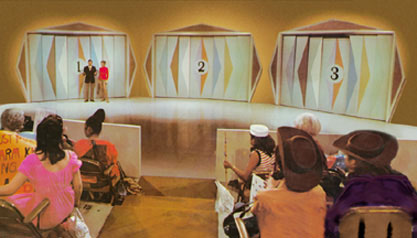
\includegraphics[width=\linewidth]{letsmakeadeal70sdoors.jpg}
%\caption{caption}\label{fig:comparison_a5}
\end{wrapfigure}
%\begin{quote}
  \emph{Suppose you are on a game show and given a choice of three doors.
    Behind one is a car; behind the others are goats. You pick door No.\,1,
    and the host, who knows what is behind them [and wouldn't open the door
    with the car], opens No.\,2, which has a goat. He then asks if you want
    to pick No.\,3. Should you switch?}
%\end{quote}

\medskip

In this exercise we'll try to answer this puzzle using the probability
calculus discussed in the lecture
notes\footnote{\url{https://portamana.org/linko.htm?w=introprob2.pdf}}.
First we'll translate the initial information and the question in the
language of probability, then we'll find the numerical values of the
requested probabilities, and finally we'll check how the answer changes if
the initial information is slightly different. Try to solve as many of the
queries below, step by step, as your time allows you to. At least skim
through the whole exercise to understand the procedure we're following. I'd
be happy if you at least tried Query~\ref{sec:lab}, the most important,
sometime in the future.

\bigskip

\setcounter{section}{-1}%
\section{Intuition}
\label{sec:preintuition}

First of all \quest{examine what your intuition tells you the answer should be},
without spending too much time thinking, just as if you were on the game
show. Examine which kind of heuristics your intuition uses. If you already
know the solution to this puzzle, try to remember what your intuition told
you the first time you faced it. Keep your observations in mind for later
on.

\bigskip

Now put your intuition aside, close its eyes, and unsheathe your analytic
skills. Let the probability calculus be your compass.


\section{Statements}
\label{sec:statement}

% First we draw a map of our puzzle, with all the main paths we have to consider:

% \medskip

\quest{Write down the \emph{statements} that we have to use in order to analyse and
  solve the puzzle.}

\medskip

If the present step is unclear or difficult, take a peek at the answer on
the next page. Make sure your answer matches the one given there before
proceeding to the next query.

\clearpage

\addsubsec{Answer}

The following \emph{statements} turn out to be enough:
\begin{align}
  \label{eq:statements}
  &\begin{aligned}
    k &\defd\text{[The general \emph{\textbf{k}}nowledge provided with the puzzle]}
    \\
    \cara&\defd\defquote{\text{The car is behind door 1}}\\
    \carb&\defd\defquote{\text{The car is behind door 2}}\\
    \carc&\defd\defquote{\text{The car is behind door 3}}\\[0.5\jot]
    \hostb&\defd\defquote{\text{The host opens door 2}}\\[0.5\jot]
    \youa&\defd\defquote{\text{You initially pick door 1}}
  \end{aligned}
\\\intertext{We can also consider additional statements, like these:}
  \label{eq:statements2}
  &\begin{aligned}
    \hosta&\defd\defquote{\text{The host opens door 1}}\\
    \hostc&\defd\defquote{\text{The host opens door 3}}
  \end{aligned}
\end{align}
but they aren't used in the solution of the problem.

\medskip

The symbols I chose (\enquote{$\cara$}, \enquote{$\hostb$}, \etc) are of
course unimportant. We could for example use \enquote{$\textit{C1}$}
instead of \enquote{$\cara$}, and so on.

\clearpage

\section{Initial probabilities}
\label{sec:init_probs}

% Next, we must locate our starting point on the map:

% \medskip

\quest{Translate the information given in the problem into initial
  probabilities having definite numerical values.} These probabilities
involve the statements found in the previous query.

\medskip

If the present step is unclear or difficult, take a peek at the answer on
the next page. Make sure your answer matches the one given there before
proceeding to the next query.

\clearpage

\addsubsec{Answer}

The initial information can be summarized in the following probabilities.

\bigskip

We're assuming that you're initially equally uncertain about where the car
is, and that your initial pick of a door doesn't change your uncertainty:
\begin{equation}
  \label{eq:probs0}
  \begin{split}
    &\p(\cara \|k) = \p(\cara\|\youa\;k) = 1/3,\\
    &\p(\carb \|k) = \p(\carb\|\youa\;k) = 1/3,\\
    &\p(\carc \|k) = \p(\carc\|\youa\;k) = 1/3.
  \end{split}
\end{equation}

The host won't open your door and won't open the door with the car. If the
car is behind door No.\,1 he has a choice between No.\,2 and 3. His options
are expressed by these probabilities:
\begin{subequations}
  \label{eq:probshost}
  \begin{equation}\label{eq:host_choice}
    \begin{gathered}
      \p(\hosta|\cara\;\youa\;k) = 0,\\
      \p(\hostb|\cara\;\youa\;k) = 1/2,\qquad
      \p(\hostc|\cara\;\youa\;k) = 1/2.
      \end{gathered}
\end{equation}
The $1/2$ in the last two probabilities expresses that we don't know which
door the host would choose to open, if he has a choice between two.

If the car is behind door No.\,2, his options are more limited:
\begin{equation}
  \begin{gathered}
    \p(\hosta|\carb\;\youa\;k) = 0,\quad
    \p(\hostb|\carb\;\youa\;k) = 0,\\
    \p(\hostc|\carb\;\youa\;k) = 1.
  \end{gathered}
\end{equation}
Similarly if  the car is behind door No.\,3:
\begin{equation}
  \begin{gathered}
    \p(\hosta|\carc\;\youa\;k) = 0,\quad
    \p(\hostb|\carc\;\youa\;k) = 1,\\
    \p(\hostc|\carc\;\youa\;k) = 0.
  \end{gathered}
\end{equation}
\end{subequations}

No matter what you or the host do, the car is surely behind one of the
doors, and it can't be behind more than one door:
\begin{equation}
  \label{eq:probscar}
  \begin{aligned}
    &\p(\cara\lor\carb\lor\carc\|\dotso\;k) = 1,\\[0.5\jot]
    &\p(\cara\;\carb\|\dotso\;k) = 
    \p(\cara\;\carc\|\dotso\;k) = 
    \p(\carb\;\carc\|\dotso\;k) = 0,\\
    &\p(\cara\;\carb\;\carc\|\dotso\;k) = 0.
  \end{aligned}
\end{equation}


\clearpage



\section{What is the question?}
\label{sec:question}

% Next, we must locate the destination we wish to reach:

% \medskip

\quest{Translate the question of the problem into probabilities which we want to
calculate.}

\medskip

If the present step is unclear or difficult, take a peek at the answer on
the next page. Make sure your answer matches the one given there before
proceeding to the next query.

\clearpage

\addsubsec{Answer}

To decide whether we should switch to door No.~3, we must first calculate
the probability that the car is behind that door and the probability that
it is behind the door we picked, No.~1, \emph{considering all the
  information we've gathered} -- especially the host's choice. We then
compare these probabilities:
\begin{equation}
  \label{eq:question}
  \p(\cara \| \hostb\;\youa\; k) = \mathord{?}\qquad
  \p(\carc \| \hostb\;\youa\; k) = \mathord{?}
\end{equation}

\clearpage


\section{Solution via Bayes's theorem}
\label{sec:question}

% Now we can use our compass. It turns out that in puzzles of this kind
% there's a shortest path. Our compass guides safely through it:

% \medskip

\quest{Find the numerical values of the probabilities identified in the
  previous query. Use Bayes's theorem in the form}
\begin{multline}
  \label{eq:bayes_hyp}
  \p(\hypa\|\data\;\info) ={}\\
  \frac{
\p(\data\|\hypa\;\info) \times \p(\hypa\|\info)
}{
\p(\data\|\hyppa\;\info) \times \p(\hyppa\|\info)
+ \p(\data\|\hyppb\;\info) \times \p(\hyppb\|\info)
}
\end{multline}
\quest{and similarly for $\hypb$. What are the \enquote{hypotheses} and the
  \enquote{data} in this problem?}

\medskip

If the present step is unclear or difficult, take a peek at the answer on
the next page. Make sure your answer matches the one given there
before proceeding to the next query.

\clearpage

\addsubsec{Answer}

We have two hypotheses: $\cara\defd{}$\defquote{the car is behind door No.\,1},
and $\carc\defd{}$\defquote{the car is behind door No.\,3}. Our data is
$\hostb$: the fact that the host chose door No.\,2. Our initial information
is the general information of the puzzle, $k$, and the fact that we
initially picked No.\,1, $\youa$. (If you're wondering \enquote{why is
  $\youa$ not part of the data?}, read below.)

\smallskip

Bayes's theorem~\eqref{eq:bayes_hyp} for  hypothesis $\cara$ in our case becomes
\begin{subequations}
  \label{eq:bayes_sol1}
\begin{multline}%[\linewidth]
  \p(\cara\|\hostb\;\youa\,k) ={}\\[0.5\jot]
  \frac{
    \p(\hostb\|\cara\;\youa\,k) \times \p(\cara\|\youa\,k)
  }{\left[ 
      \!\begin{multlined}[0.9\linewidth]
        \p(\hostb\|\cara\;\youa\,k) \times \p(\cara\|\youa\,k)
        +{}\\ \p(\hostb\|\carc\;\youa\,k) \times \p(\carc\|\youa\,k)
      \end{multlined} \right]
  }\label{eq:bayes_sol1a}
\end{multline}
and using the numerical values of the initial
probabilities~\eqref{eq:probs0}--\eqref{eq:probscar} we find
\colorlet{shadecolor}{myblue}
\begin{snugshade}%\vspace{-1.5em}
\begin{equation}
\p(\cara\|\hostb\;\youa\,k) =
        \frac{ \frac{1}{2} \times \frac{1}{3} }{ \frac{1}{2} \times
          \frac{1}{3} +1 \times \frac{1}{3} } = \frac{1}{3}.
  \end{equation}
\end{snugshade}
\end{subequations}
\noindent Bayes's theorem for  hypothesis $\carc$  becomes
\begin{subequations}
  \label{eq:bayes_sol3}
\begin{multline}%[\linewidth]
  \p(\carc\|\hostb\;\youa\,k) ={}\\[0.5\jot]
  \frac{
    \p(\hostb\|\carc\;\youa\,k) \times \p(\carc\|\youa\,k)
  }{\left[ 
      \!\begin{multlined}[0.9\linewidth]
        \p(\hostb\|\cara\;\youa\,k) \times \p(\cara\|\youa\,k)
        +{}\\ \p(\hostb\|\carc\;\youa\,k) \times \p(\carc\|\youa\,k)
      \end{multlined} \right]
  }
\end{multline}
and replacing the numerical values of the initial probabilities we find
\colorlet{shadecolor}{myblue}
\begin{snugshade}
  \begin{equation}
    \p(\carc\|\hostb\;\youa\,k) =
    \frac{
      1 \times \frac{1}{3}
    }{
      \frac{1}{2} \times \frac{1}{3}
      +1 \times \frac{1}{3}
    }
    = \frac{2}{3}.
  \end{equation}
\end{snugshade}
\end{subequations}
\noindent \textbf{That is, the car is more likely to be behind door No.\,3!
\emph{We should therefore switch}.}

\medskip

Let's see if Bayes's theorem correctly finds also the obvious: it's
impossible that the car is behind door No.\,2:
\begin{subequations}
  \label{eq:bayes_sol2}
\begin{multline}%[\linewidth]
  \p(\carb\|\hostb\;\youa\,k) ={}\\[0\jot]
  \frac{
    \p(\hostb\|\carb\;\youa\,k) \times \p(\carb\|\youa\,k)
  }{\left[ 
      \!\begin{multlined}[0.9\linewidth]
        \p(\hostb\|\cara\;\youa\,k) \times \p(\cara\|\youa\,k)
        +{}\\ \p(\hostb\|\carb\;\youa\,k) \times \p(\carb\|\youa\,k)
        +{}\\[-\jot] \p(\hostb\|\carc\;\youa\,k) \times \p(\carc\|\youa\,k)
      \end{multlined} \right]
  }
\end{multline}
and substituting the initial probabilities:
\begin{equation}
    \p(\carb\|\hostb\;\youa\,k) =
      \frac{
      0 \times \frac{1}{3}
      }{
      \frac{1}{2} \times \frac{1}{3}
      +0 \times \frac{1}{3}
      +1 \times \frac{1}{3}
      }
      = 0,
    \end{equation}
\end{subequations}
a reassuring result.

\bigskip

In choosing what our \enquote{data} are, you may have asked yourself the
following question: Should my initial door pick, $\youa$, be included in
the \enquote{data}? It's a great question. Your own door choice came as no
surprise to you, so it seems more reasonable to consider it as part of the
\enquote{other info}, as we did above.

\emph{\textbf{But the important point is this:}} there wouldn't be anything
wrong in including your door pick among the \enquote{data}. In fact,
\emph{Bayes's theorem would give us exactly the same numerical result even
  if we took \enquote{$\hostb\;\youa$} as \enquote{$\data$}}. This equality
is a result of the self-consistency of the probability calculus.

In this case Bayes's theorem for $\cara$ takes this form:
\begin{multline}%[\linewidth]
  \p(\cara\|\hostb\;\youa\,k) ={}\\[0\jot]
  \frac{
    \p(\hostb\;\youa\|\cara\;k) \times \p(\cara\| k)
  }{\left[ 
      \!\begin{multlined}[0.9\linewidth]
        \p(\hostb\;\youa\|\cara\;k) \times \p(\cara\| k)
        +{}\\ \p(\hostb\;\youa\|\carc\;k) \times \p(\carc\|k)
      \end{multlined} \right]
  }\label{eq:bayes_alter}
\end{multline}
and you see that it involves probabilities that we don't have yet, for
example $\p(\hostb\;\youa\|\cara\;k)$. We'd need to first calculate these
probabilities from our initial ones~\eqref{eq:probs0}--\eqref{eq:probscar},
using the five probability rules. It would be a bit of extra work (feel
free to do this as an extra query). After this extra calculations you'd
find that Bayes's formula~\eqref{eq:bayes_alter} above actually simplifies
to~\eqref{eq:bayes_sol1a}! So, a different choice of what's \enquote{data}
wouldn't be wrong but would be less convenient, leading to more
calculations.

This is a great feature, though: Even if you do your analysis in a slightly
roundabout way, the probability calculus will lead you to the correct
answer anyway -- provided you follow all its rules exactly. Again, this
happens because the probability calculus is just an extension of logic.

Finally, note that whether we consider your door pick, $\youa$, as part of
the data or of the initial information, its specification is essential for
solving the problem: if you had picked another door, the host's options
would have been different. 

\clearpage


\section{Let's educate our intuition}
\label{sec:intuition}

% We've arrived at our destination. It may look unfamiliar and not as we were
% expecting it to look like (we've never been here before).

% \medskip

Does the answer you just found agree with your initial intuition? Most
people find the correct answer counter-intuitive. I did. If your initial
intuition told you differently, try to educate it by examining the results
from Bayes's formulae~\eqref{eq:bayes_sol1}--\eqref{eq:bayes_sol2}. There's
no right or wrong answer. You can see my personal analysis on the next
page. People's intuitions often work in different ways, so the only person
who can educate your intuition is you.

Proceed next to query~\ref{sec:inside_info_car} on
page~\pageref{sec:inside_info_car}.



\clearpage

\addsubsec{\emph{My} answer}

% I personally don't like explanations such as \enquote{chance} and \enquote{random}
% out of the way, because they're never helpful. If someone says
% \enquote{this happens by chance} -- or, with a technical disguise,
% \enquote{this is \emph{stochastic}} -- all they mean is \enquote{I don't
%   know what mechanism makes this happen}: an honest statement, but with no
% usefulness whatsoever.

Where does the final difference between the credibilities of the two
hypotheses $\cara$ and $\carc$ come from? Bayes's
formulae~\eqref{eq:bayes_sol1} and \eqref{eq:bayes_sol3} show that the only
difference is in the plausibilities of the host's actions given the two
hypotheses and given that you picked door No.\,1:
\begin{equation}
  \label{eq:host_options}
      \p(\hostb|\cara\;\youa\;k) = 1/2,\qquad
    \p(\hostb|\carc\;\youa\;k) = 1.
\end{equation}
The host's choice gave us \emph{information} that led to a change in the
credibilities of the two hypotheses. The most obvious piece of information
given by the host's choice is that the car can't be behind door No.\,2: we
know that it can't as soon as the host starts to open that door. If the car
had been there, the host couldn't have opened that door:
\begin{equation}
  \label{eq:host_no_2}
  \p(\hostb|\carb\;\youa\;k) = 0.
\end{equation}
But this obvious, large piece of information -- so important that it
immediately makes the hypothesis $\carb$ impossible and excluded at the
outset -- is \emph{not} used in Bayes's formulae~\eqref{eq:bayes_sol1} and
\eqref{eq:bayes_sol3}. So these formulae are telling us that the host's
action contains \emph{additional}, subtler pieces of useful information.

In fact the probabilities~\eqref{eq:host_options} tell us that it's more
likely that the host opens door No.\,2 under the hypothesis $\carc$ (where
it's the only possible action for him) than under the hypothesis $\cara$
(where he has two possible choices). The observation of $\hostb$ therefore
provides slightly stronger evidence for $\carc$ than for $\cara$. Or we can
say that $\carc$ has slightly more \enquote{explanatory power} for $\hostb$ than
$\cara$ does. Since the two hypotheses were initially equally plausible,
the new evidence now makes $\cara$ less plausible. Not impossible, just
less plausible. This reasoning is a sort of softened version of the logical
impossibility of hypothesis $\carb$; it shows that the plausibility
calculus is an extension of formal logic \citep[take a look
at][]{hailperin1984,hailperin1991,hailperin1996}.
% Sadly, many statisticians are unaware of the logicians' work}.


When I first faced this puzzle I didn't think about these slightly
different informational connections between $\hostb$ on one side and
$\cara$, $\carc$ on the other. They were eclipsed by the much stronger
logical connection between $\hostb$ and $\carb$: \enquote{he opens that
  door -- no car there then; that's all there is to it}. So what my
intuition learned from the probability calculation is not to exult and stop
searching just because a very strong and important piece of information is
revealed: there may be additional crumbs of information hiding around, and
together they may lead to far stronger conclusions.\footnote{As The Wolf
  concisely puts it in \emph{Pulp Fiction}: \enquote{Well, let's not start
    sucking each other's dicks quite yet}
  (\url{https://www.youtube.com/watch?v=7zfbkhj8D0c}, 01:00).} This is what
happens, for example, with magnetic-resonance imaging: the probability
calculus is able to gather and assemble from the signal so many numerous
pieces of information, each one invisible to the naked eye, that the final
frequency estimate is \emph{orders of magnitude} better than obtained from
a Fourier transform. I invite you to read pages 23--24 of Bretthorst
\citey{bretthorst1988} for an insightful discussion of this phenomenon.

The strength of the probability calculus is that it automatically keeps
every shred of information into account (unless we too hurriedly skip
steps, deluding ourselves to have found everything there was to be found).


\clearpage

%\plainfancybreak{3\baselineskip}{1}{*\quad*\quad*}
\fancybreak*{*\quad*\quad*}

The solution we found depends on our \emph{symmetric} states of ignorance
regarding the placement of the car, formulae~\eqref{eq:probs0}, and
regarding the host's decision when he has a choice between two doors,
formulae~\eqref{eq:host_choice}. Let's examine how the credibilities change
if we have some additional information.


\section{Inside information about the car}
\label{sec:inside_info_car}

Let's consider our puzzle from the point of view of a different state of
knowledge $k'$. You have a friend who works backstage. They secretly tell
you (hey, that's cheating!) that they saw some large object -- probably the
car -- being moved towards the left side (door No.\,1). Because of this
information you think it's more likely that the car is placed somewhat
towards the left (door No.\,1) than the right (door No.\,3). Let's express
this information by subtracting a positive amount $x$ from the initial
probability of $\carc$ and giving it to $\cara$:%
\setlength{\intextsep}{0.1ex}% with wrapfigure
\begin{wrapfigure}{l}{0.35\linewidth}% with wrapfigure
\centering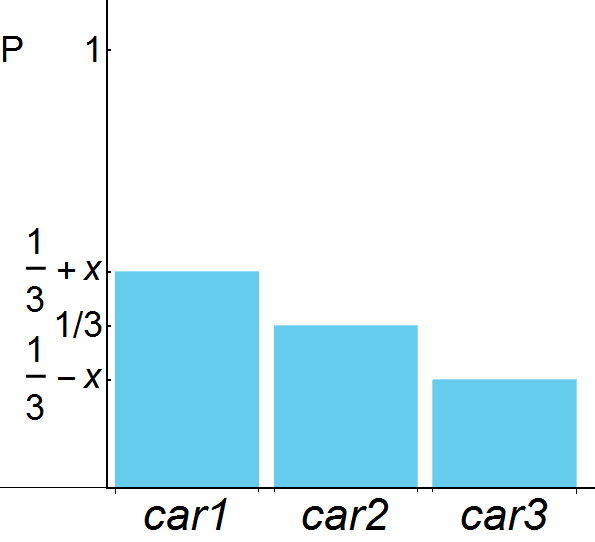
\includegraphics[width=\linewidth]{carnew.png}%
\vspace{-3em}%  
%\caption{caption}\label{fig:comparison_a5}
\end{wrapfigure}
\begin{equation}
  \label{eq:new_probscar}
    \begin{split}
    &\p(\cara \|k) = \p(\cara\|\youa\;k') = \tfrac{1}{3} +x,\\
    &\p(\carb \|k) = \p(\carb\|\youa\;k') = \tfrac{1}{3},\\
    &\p(\carc \|k) = \p(\carc\|\youa\;k') = \tfrac{1}{3} -x,
  \end{split}
\end{equation}
so that we have a linear decrease from door No.\,1 to door No.\,3.
Obviously $x\le 1/3$, because we can't have negative probabilities.

In our previous calculation we saw that the host's opening of No.\,2 gives
more evidence to $\carc$ than to $\cara$. Now we have initially more
evidence for $\cara$ than for $\carc$. It's possible that these two pieces
of evidence balance each other out.

\medskip

\quest{Calculate for which value $x$ it doesn't matter whether you switch
  or not after the host opens No.\,2.}

\medskip

If the present step is unclear or difficult, take a peek at the answer on
the next page. Then proceed to the next query.

\clearpage

\addsubsec{Answer}

The alternative state of knowledge $k'$ differs from $k$ only in the values
of the initial probabilities for the car's position:
formulae~\eqref{eq:new_probscar} instead of~\eqref{eq:probs0}. Bayes's
formulae~\eqref{eq:bayes_sol1}--\eqref{eq:bayes_sol3} for the final
probabilities for the car's position still apply, but with the new values
of the initial probabilities. We have
\begin{align}
  &\p(\cara\|\hostb\;\youa\,k') =
    \frac{ \frac{1}{2} \times \bigl( \frac{1}{3} +x \bigr) }{
    \frac{1}{2} \times \bigl( \frac{1}{3} +x \bigr) +
    1 \times \bigl( \frac{1}{3} -x \bigr)}
  \\
  &\p(\carc\|\hostb\;\youa\,k') =
    \frac{ 1 \times \bigl( \frac{1}{3} +x \bigr) }{
    \frac{1}{2} \times \bigl( \frac{1}{3} +x \bigr) +
    1 \times \bigl( \frac{1}{3} -x \bigr)}
\end{align}

The query asks for which value of $x$ it doesn't matter whether we switch
or not. This means that the final probabilities for $\cara$ and $\carc$,
\eqref{eq:bayes_sol1} and \eqref{eq:bayes_sol3}, are equal. Let's therefore
equate the two probabilities above. Note that the two fractions have the
same denominator (which is different from zero), so we can just equate the
numerators:
\colorlet{shadecolor}{myblue}
\begin{snugshade}
\begin{equation}
  \label{eq:equate_prob1}
  \frac{1}{2} \times \biggl( \frac{1}{3} +x \biggr) =
  1 \times \biggl( \frac{1}{3} +x \biggr)
  \quad\implies\quad
  x=\frac{1}{9}.
\end{equation}
\end{snugshade}
This means that if the initial credibilities for the car's position are
\begin{equation}
  \label{eq:new_probscar_equal}
    \begin{split}
    &\p(\cara \|k) = \p(\cara\|\youa\;k') = 4/9,\\
    &\p(\carb \|k) = \p(\carb\|\youa\;k') = 3/9,\\
    &\p(\carc \|k) = \p(\carc\|\youa\;k') = 2/9,
  \end{split}
\end{equation}
then, after the host opens door No.\,2, we are equally uncertain whether
the car is behind No.\,1 or No.\,2, and so it doesn't matter whether we
switch or not.

In general, if $x<1/9$ we should switch because the credibility of $\carc$
is higher, and if $x>1/9$ we should keep No.\,1 because the credibility of
$\cara$ is higher.


\clearpage

\section{Inside information about the host}
\label{sec:inside_host}

In the previous query we had inside information about the car's position.
Now let's consider yet another state of knowledge $k''$, in which we have
inside information about the host instead. Your friend backstage secretly
tells you that the host recently had a leg injury and feels some pain when
walking. He still wants to present the show, but will limit his walking to a
minimum. Since the host initially always stands close to door No.\,1, this
means that, given the choice to open door No.\,2 or No.\,3 (this happens
when you've picked No.\,1 and the car is there too) he will likely
choose the closest: No.\,2. This knowledge leads us to assign unequal
probabilities for $\hostb$ and $\hostc$ conditional on $\cara\;\youa$.
Instead of the values~\eqref{eq:probshost}, let's say that the plausibility
that the host opens No.\,2 if the car is behind No.\,1 is $y$:
  \begin{equation}\label{eq:host_choice_new}
    \begin{gathered}
      \p(\hosta|\cara\;\youa\;k) = 0,\\
      \p(\hostb|\cara\;\youa\;k) = y,\qquad
      \p(\hostc|\cara\;\youa\;k) = 1-y.
      \end{gathered}
\end{equation}
This affects the values of the probabilities for the car after the host
opens door No.\,2.

\medskip

\quest{Calculate for which value of $y$ (if any) it doesn't matter whether
  you switch or not after the host opens No.\,2.}

\medskip

If the present step is unclear or difficult, take a peek at the answer on
the next page. Make sure your answer matches the one given there before
proceeding to the next -- and final! -- query.



\clearpage

\addsubsec{Answer}



The alternative state of knowledge $k''$ differs from $k$ only in the
values of the probabilities for the host choice: instead of
\eqref{eq:host_choice} we have now~\eqref{eq:host_choice_new}. Bayes's
formulae for the final probabilities of $\cara$ and $\carc$ still hold, but
we now have the values
\begin{align}
  &\p(\cara\|\hostb\;\youa\,k'') =
        \frac{ y \times \frac{1}{3} }{ y \times
          \frac{1}{3} +1 \times \frac{1}{3} },
\\
  &\p(\carc\|\hostb\;\youa\,k'') =
        \frac{ 1 \times \frac{1}{3} }{ y \times
          \frac{1}{3} +1 \times \frac{1}{3} }.
\end{align}

These two probabilities are equal if
\colorlet{shadecolor}{myblue}
\begin{snugshade}
\begin{equation}
  \label{eq:equate_prob2}
  y + \frac{1}{3} =
  1 \times \frac{1}{3}
  \quad\implies\quad
  y=1.
\end{equation}
\end{snugshade}
This means that it doesn't matter whether we switch only if we're
\emph{absolutely certain} that the host would never open door No.\,3 when
he has the choice between that and No.\,2 (he must be in a lot of pain!).
Otherwise, it's still best to switch.


\clearpage

\section{Let's make a deal in your research!}
\label{sec:lab}

Through the previous queries we've seen that the Monty Hall problem is just
another example of calculating the probabilities of some hypotheses
(\enquote{where's the car?}) given some observations or data (\enquote{the
  host chose that specific door}) and background information (the rules of
the game and that you picked No.\,1). The general steps we've taken here
would apply identically in a scientific problem. The only difference would
be in the number of hypotheses and in the determination of the initial
probabilities.


\quest{\begin{enumerate}[label=(\alph*)]
\item Consider a problem of hypothesis comparison that you're facing in
  your research at the moment, or that you faced recently. Simplify it a little.
\item Simplify the number of hypotheses to two or three.
\item Write down the values of initial credibilities of these hypotheses
  (before you did your experiments); choose values that seem to correctly
  reflect your initial beliefs.
\item \label{item:prob_data_hyp}Write down approximate/\enquote{toy} values of the
  probabilities of the result you obtained, conditional on each hypothesis;
  choose values that seem to correctly reflect the connection between
  hypothesis and result, but don't overthink too much.
\item Calculate the values of the credibilities of the hypotheses in view
  of your result, using Bayes's theorem~\eqref{eq:bayes_hyp} with the
  probabilities you wrote down in the two steps above.
\end{enumerate}
}

\medskip

Obviously you can't trust the result of this analysis in a quantitative
(maybe not even qualitative) way, because the probabilities you wrote down
in step~\ref{item:prob_data_hyp} may not correctly reflect sensitive
experimental details: you'd need to analyse that in much more detail,
probably using numerical software.

Yet, you have just done a first rough Bayesian analysis of a concrete
scientific problem.


\clearpage

\addsec{Optional query: the probability calculus}
\label{sec:bonus}

In the
lecture\footnote{\url{https://portamana.org/linko.htm?w=introprob2.pdf}} we
saw that Bayes's theorem is simply a very convenient summary of a sequence
of calculations that only involve the five probability rules. If you're
curious about the step-by-step calculation, feel free to try it as we did
during the lecture in the breast-cancer problem\ibid\ (pdf page~98). Use the probability rules
and shortcuts from the slides, and follow the roadmap shown in the next
page. \mr{Solid red lines}: \enquote{and} rule; \mb{dashed blue lines}:
\enquote{or} ($\lor$) rule.

%\thispagestyle{empty}
\begin{figure}[p]
  \centering
  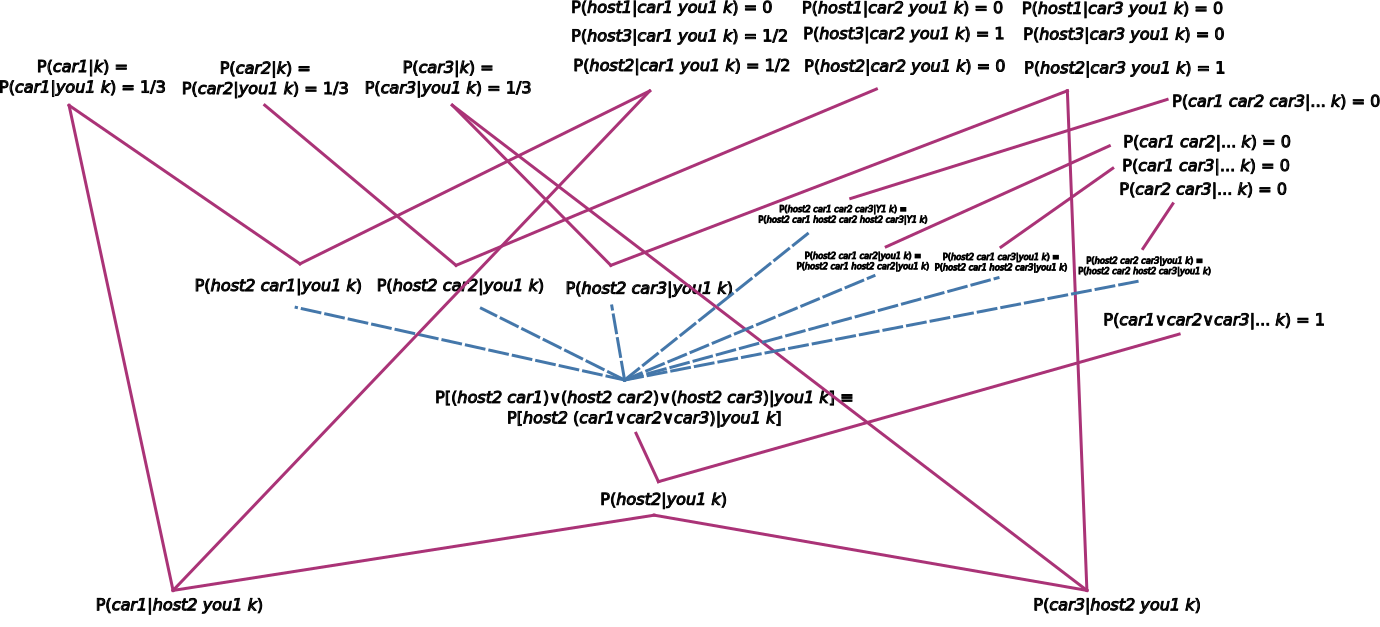
\includegraphics[width=1.06\textheight,angle=-90]{prob_tree_monty2.png}%
\end{figure}



%\clearpage
%\renewcommand*{\appendixpagename}{}
%\renewcommand*{\appendixname}{}
%\appendix




%%%%%%%%%%%%%%%%%%%%%%%%%%%%%%%%%%%%%%%%%%%%%%%%%%%%%%%%%%%%%%%%%%%%%%%%%%%%
%%% Epigraph
%%%%%%%%%%%%%%%%%%%%%%%%%%%%%%%%%%%%%%%%%%%%%%%%%%%%%%%%%%%%%%%%%%%%%%%%%%%%
% \asudedication{\small ***}
% \vspace{\bigskipamount}
% \setlength{\epigraphwidth}{.7\columnwidth}
% %\epigraphposition{flushright}
% \epigraphtextposition{flushright}
% %\epigraphsourceposition{flushright}
% \epigraphfontsize{\footnotesize}
% \setlength{\epigraphrule}{0pt}
% %\setlength{\beforeepigraphskip}{0pt}
% %\setlength{\afterepigraphskip}{0pt}
% \epigraph{\emph{text}}{source}



%%%%%%%%%%%%%%%%%%%%%%%%%%%%%%%%%%%%%%%%%%%%%%%%%%%%%%%%%%%%%%%%%%%%%%%%%%%%
%%% BEGINNING OF MAIN TEXT
%%%%%%%%%%%%%%%%%%%%%%%%%%%%%%%%%%%%%%%%%%%%%%%%%%%%%%%%%%%%%%%%%%%%%%%%%%%%



% \[
%   \begin{tikzcd}
%       M_{n,n}(\CC) \arrow{r}{R'_{a}(\Hat{U})} & M_{n,n}(\CC)
%     \\
%     L(\mathcal{H}) \arrow{r}{\Hat{U}} \arrow[swap]{d}{R_*}\arrow[swap]{u}{R'_*} & L(\mathcal{H}) \arrow{d}{R_*}\arrow{u}{R'_*} \\
%       M_{n,n}(\CC) \arrow{r}{R_{a}(\Hat{U})} & M_{n,n}(\CC)
%   \end{tikzcd}
% \]

% \[
%   \begin{tikzcd}
%       \CC^n \arrow{r}{R'_*(A)} & \CC^n
%     \\
%     \mathcal{H} \arrow{r}{A} \arrow[swap]{d}{R}\arrow[swap]{u}{R'} & \mathcal{H} \arrow{d}{R}\arrow{u}{R'} \\
%       \CC^n \arrow{r}{R_*(A)} & \CC^n
%   \end{tikzcd}
% \]


% \[
%   \begin{tikzcd}
%     \mathcal{H} \arrow{r}{A} \arrow[swap]{d}{R} & \mathcal{H} \arrow{d}{R} \\
%       \CC^n \arrow{r}{R_*(A)} & \CC^n
%   \end{tikzcd}
% \]

%%\setlength{\intextsep}{0.5ex}% with wrapfigure
%\begin{figure}[p!]%{r}{0.4\linewidth} % with wrapfigure
%  \centering\includegraphics[trim={12ex 0 18ex 0},clip,width=\linewidth]{maxent_saddle.png}\\
%\caption{caption}\label{fig:comparison_a5}
%\end{figure}% exp_family_maxent.nb


%%%%%%%%%%%%%%%%%%%%%%%%%%%%%%%%%%%%%%%%%%%%%%%%%%%%%%%%%%%%%%%%%%%%%%%%%%%%
%%% Acknowledgements
%%%%%%%%%%%%%%%%%%%%%%%%%%%%%%%%%%%%%%%%%%%%%%%%%%%%%%%%%%%%%%%%%%%%%%%%%%%% 
\iffalse
\begin{acknowledgements}
  \ldots to Mari \amp\ Miri for continuous encouragement and affection, and
  to Buster Keaton and Saitama for filling life with awe and inspiration.
  To the developers and maintainers of \LaTeX, Emacs, AUC\TeX, Open Science
  Framework, Python, Inkscape, Sci-Hub for making a free and unfiltered
  scientific exchange possible.
%\rotatebox{15}{P}\rotatebox{5}{I}\rotatebox{-10}{P}\rotatebox{10}{\reflectbox{P}}\rotatebox{-5}{O}.
\sourceatright{\autanet}
\end{acknowledgements}
\fi

%%%%%%%%%%%%%%%%%%%%%%%%%%%%%%%%%%%%%%%%%%%%%%%%%%%%%%%%%%%%%%%%%%%%%%%%%%%%
%%% Appendices
%%%%%%%%%%%%%%%%%%%%%%%%%%%%%%%%%%%%%%%%%%%%%%%%%%%%%%%%%%%%%%%%%%%%%%%%%%%% 
\clearpage
% %\renewcommand*{\appendixpagename}{Appendix}
% %\renewcommand*{\appendixname}{Appendix}
% %\appendixpage
% \appendix

%%%%%%%%%%%%%%%%%%%%%%%%%%%%%%%%%%%%%%%%%%%%%%%%%%%%%%%%%%%%%%%%%%%%%%%%%%%%
%%% Bibliography
%%%%%%%%%%%%%%%%%%%%%%%%%%%%%%%%%%%%%%%%%%%%%%%%%%%%%%%%%%%%%%%%%%%%%%%%%%%% 
\defbibnote{prenote}{{\footnotesize (All references are available in the
    \texttt{cited\_literature} folder.)\par}}
% \defbibnote{postnote}{\par\medskip\noindent{\footnotesize% Note:
%     \arxivp \mparcp \philscip \biorxivp}}

\printbibliography[%prenote=prenote%,postnote=postnote
]

\end{document}

%%%%%%%%%%%%%%%%%%%%%%%%%%%%%%%%%%%%%%%%%%%%%%%%%%%%%%%%%%%%%%%%%%%%%%%%%%%%
%%% Cut text (won't be compiled)
%%%%%%%%%%%%%%%%%%%%%%%%%%%%%%%%%%%%%%%%%%%%%%%%%%%%%%%%%%%%%%%%%%%%%%%%%%%% 


%%% Local Variables: 
%%% mode: LaTeX
%%% TeX-PDF-mode: t
%%% TeX-master: t
%%% End: 
